\documentclass[12pt]{article}

\setlength\parindent{0pt}
\newcommand{\myt}[1]{\textbf{\underline{#1}}}

\usepackage{mathtools}
\usepackage{amssymb}
\usepackage{tikz,ifthen,amsmath,amssymb,fancyhdr,comment,lastpage}

\title{\vspace{-15ex}Module 4 - Dictionaries and Balanced Search Trees\vspace{-1ex}}
\date{June 2nd, 2015}
\author{Graham Cooper}

\begin{document}
	\maketitle
	\section*{Dictionaries}
	\begin{itemize}
		\item An ADT
		\item Data (key, value) pairs
		\item operations: search, insert, delete
	\end{itemize}
	
	Data Structures for Dictionaries:
	\begin{itemize}
		\item unsorted array or linked list
		\begin{itemize}
			\item search: O(n)
			\item insert: O(1)
			\item Delete: O(n)
		\end{itemize}
		\item sorted array
		\begin{itemize}
			\item search - binary search O(logn)
			\item insert O(n)
			\item delete O(n)
		\end{itemize}
		
	\end{itemize}
	
	\subsection{BST}
	
	\begin{center}\begin{tikzpicture}[
		level distance=45 pt,
		every node/.style={circle,draw},
		level 1/.style={sibling distance=200 pt},
		level 2/.style={sibling distance=100 pt},
		level 3/.style={sibling distance=60 pt}
		]
		\node {20}
		child {node {10}
			child {node {5}
				child {node {1}}
				child {node {8}}
			}
			child {node {15}
				child [missing]
				child {node {16}}
			}
		}
		child {node {50}
			child [missing]
			child {node{70}
				child {node {60}}
				child {node {80}}
			}	
		}
		;
		\end{tikzpicture}\end{center}
	
	Insert 6\\
	
	\begin{center}\begin{tikzpicture}[
		level distance=45 pt,
		every node/.style={circle,draw},
		level 1/.style={sibling distance=200 pt},
		level 2/.style={sibling distance=100 pt},
		level 3/.style={sibling distance=60 pt}
		]
		\node {20}
		child {node {10}
			child {node {5}
				child {node {1}}
				child {node {8}
					child {node{6}}
					child [missing]	
				}
			}
			child {node {15}
				child [missing]
				child {node {16}}
			}
		}
		child {node {50}
			child [missing]
			child {node{70}
				child {node {60}}
				child {node {80}}
			}	
		}
		;
		\end{tikzpicture}\end{center}
	
	Delete in a BST\\
	\begin{itemize}
		\item if n is a leaf - just delete it
		\item if n is a node with one child, replace it with its child
		\item if n has two children, replace with the predecessor (rightmost on the left) or sucessor (left most)
	\end{itemize}
	
	\section*{Fun with AVL trees (control)}
	%%
	%%	\begin{center}\begin{tikzpicture}[
	%%		level distance=45 pt,
	%%		every node/.style={circle,draw},
	%%		level 1/.style={sibling distance=100 pt},
	%%		level 2/.style={sibling distance=100 pt},
	%%		level 3/.style={sibling distance=100 pt}
	%%		]
	%%		\node {50}
	%%		child {node {20}
	%			child {node {10}
	%				child {node {8}}
	%				child {node {8}}
	%			}
	%			child {node {30}}
	%		}
	%		child {node {70}
	%			child [missing]
	%			child {node{70}
	%				child {node {60}
	%					child {node {55}}
	%					child {node {65}
	%						child {node {62}
	%							child [missing]
	%							child {node {63}}
	%						}
	%					child [missing]
	%					}
	%				}
	%				child {node {80}
	%					child {node {75}
	%						child {node {72}}
	%						child [missing]
	%						}
	%					child {node {85}}
	%				}
	%			}	
	%		}
	%		;
	%		\end{tikzpicture}\end{center}
		
	\myt{insert(y)}\\
	- insert as a leaf like usual bst\\
	----Move up, update balance factors\\
	------ if  x.balance factor $\in$ \{-2, 2\}\\
	-------- fin(x)\\
	Fin is called at most once after that bf, are all fixed (no need to update higher levels)\\
	
	\myt{fin(x)}\\
	if x.bf = -2 (too heavy on the left)\\
	\{
	-- if x.left.bf = 1 then\\
	---- x.left $\rightarrow$ rotate(left)\\
	-- n $\rightarrow$ rotate Right
	\}\\
	
	if x.bf = +2 (too heavy on right)\\
	\{\\
	-- if x.right.bf = -1\\
	---- x.right $\rightarrow$ rotateRight\\\
	-- x $\rightarrow$ rotateLeft()\\
	\}\\
	
	\myt{Delete(j)}\\
	-- as usual BST, replcae with successor/predecessor\\
	-- move from location of seccessor, predecessor\\
	-- -- move up\\
	-- -- -- if x.bf $\leftarrow$ \{-2,2\}\\
	-- -- -- -- fin(x)\\
	
	fin may be called log(n) times because the height changes.\\
	
	\myt{insertion}\\
	-- Insert as a usual BST\\
	-- -- O(height)\\
	-- move up check balance factor, apply fin() if neccessary\\
	-- time for fin $\rightarrow$ O(1)\\
	In total, time for insert: $\Theta$(height)\\
	
	\myt{Height of AVL:}\\
	let N(h) denote the minumum number of nods in an AVL tree with height h.\\
	N(h) = \\
	0 if h = -1\\
	1 if h = 0\\
	N(h-1) + N(h-2) + 1 else\\
	
	N(h) = fionacci(h+3) - 1\\
	= roof($\frac{p^{h+3}}{5}) - 1$\\
	where p = $\frac{1 + \sqrt{5}}{2}$\\
		
	\section*{B-Tree (beautiful tree)}
		
	\begin{center}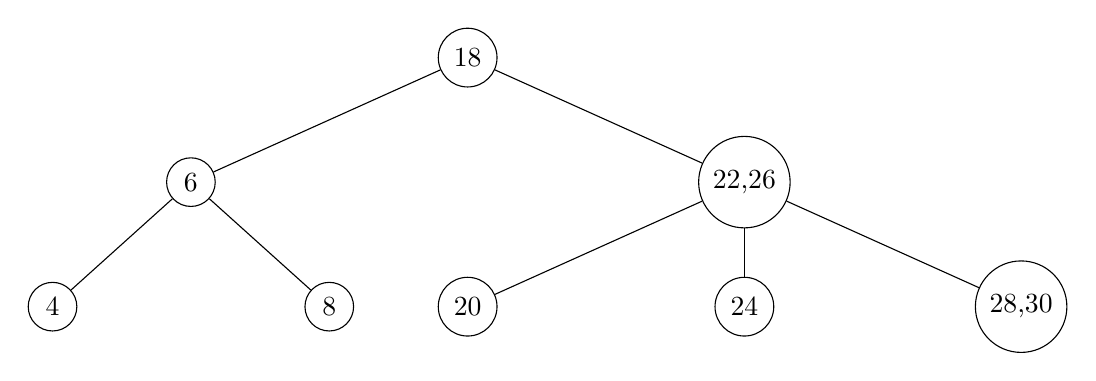
\begin{tikzpicture}[
		level distance=45 pt,
		every node/.style={circle,draw},
		level 1/.style={sibling distance=200 pt},
		level 2/.style={sibling distance=100 pt},
		level 3/.style={sibling distance=60 pt}
		]
		\node {18}
		child {node {6}
			child {node {4}
			}
			child {node {8}
			}
		}
		child {node {22,26}
			child {node {20}}
			child {node{24}}
			child {node {28,30}}
			}	
		
		;
	\end{tikzpicture}\end{center}

	An (a,b) tree B-Tree\\
	\begin{enumerate}
		\item An ordered tree
		\item Each internal node has at least a, and at most b children, root has at least 2, at most b children
		\item A node with k children $\rightarrow$ k-1 key value pairs\\
				-- An (roof($\frac{u}{2}, u))$ B-tree is order u B-tree, eg u = 2$\rightarrow$ order b-tree $\rightarrow$ A(2,3)-tree
	\end{enumerate}
	
	\myt{Insertion}\\
	--Insert at a leaf
	-- overfilled noes send the middle key to the parent and split
	
	\myt{Deletion}\\
	-- As BST, the removed key is replaced by successor/predeccesor (which is a leaf)\\
	-- if a node becomes underloaded\\
	-- -- if $\exists$ a sibling with an extra key (more than 'a' keys)\\
	-- -- -- take the key from parent and parent gets a key from the sibling.\\
	
\end{document}
